\documentclass[11pt,a4paper]{article}

\usepackage[margin=1in]{geometry}
\usepackage{amsmath}
\usepackage{booktabs}
\usepackage{tabularx}
\usepackage{graphicx}
\usepackage{xcolor}
\usepackage{fancyhdr}
\usepackage{tikz}
\usetikzlibrary{arrows.meta,positioning,calc}
\usepackage[colorlinks=true,linkcolor=black,urlcolor=blue,citecolor=black]{hyperref}

\definecolor{good}{rgb}{0.0,0.45,0.0}
\definecolor{warn}{rgb}{0.72,0.33,0.0}

\pagestyle{fancy}
\fancyhf{}
\fancyhead[L]{\small CSE 406 --- Project 20}
\fancyhead[R]{\small Demonstration Report}
\fancyfoot[C]{\thepage}
\renewcommand{\headrulewidth}{0.4pt}

\newcommand{\code}[1]{\texttt{#1}}

\begin{document}

%======================================================================
\begin{center}
{\LARGE\bfseries Wi-Fi Password Cracking --- Demonstration Report}\\[0.35em]
{\large Project 20 \quad$\cdot$\quad One offline tool, three attacks, on captured pcap files}\\[0.7em]
\begin{tabular}{rl}
Students: & Mohammad Saifuzzaman (2105088) \\
          & Sayaad Muzahid Masfi (2105066) \\
Section / Group: & B1 --- Group 3 \\
Course: & CSE 406 --- Computer Security \\
\end{tabular}
\end{center}

\noindent\rule{\textwidth}{0.4pt}

\begin{quote}
\small\textbf{Scope and honesty statement.} This project is a \emph{defensive, offline}
exercise. The tool reads captured \code{pcap} files and recovers WPA2-PSK passphrases from
them; it never touches a live network --- no radio, no packet injection, no deauthentication,
no live traffic. Per the supervisor's instruction, the attacks run on captured pcap files, and
public sample captures from the Internet are acceptable input. Every number, transcript, and
table in this report is real output produced by our own tool on the machines named; the
commands to reproduce each one are listed in Section~\ref{sec:repro}. Nothing in this report is
estimated unless it is explicitly labelled ``calculated,'' and where a number is calculated
rather than executed we say so and give the formula.
\end{quote}

%======================================================================
\section{What we built}

We wrote one tool, \code{wpacrack} (Python, standard library only --- no aircrack-ng, no
Hashcat, no scapy), that runs \textbf{three distinct password-cracking attacks} against
captured WPA2-PSK handshakes, plus a defense analyzer. All three attacks share a single
cryptographic core, so this is genuinely ``multiple attacks on one setup'' rather than three
separate programs. The three attacks differ in \emph{what they verify a guess against} and/or
\emph{where the candidate guesses come from}:

\begin{center}
\begin{tabularx}{\textwidth}{@{}l l X@{}}
\toprule
\textbf{Attack} & \textbf{Candidate source} & \textbf{How a guess is confirmed} \\
\midrule
1. Handshake MIC & wordlist & derive the PTK, recompute the EAPOL Key MIC, compare \\
2. PMKID         & wordlist & recompute $\text{PMKID}=\text{HMAC-SHA1}(\text{PMK},\ldots)$; needs only Message~1 \\
3. Mask / brute  & mask over \code{?d ?l ?u ?s ?a} tokens & same two verifiers; candidates generated from the mask instead of a wordlist \\
\bottomrule
\end{tabularx}
\end{center}

\noindent The command-line surface is a single entry point with seven subcommands:
\code{mic}, \code{pmkid}, \code{mask} (the three attacks); \code{analyze}, \code{policy},
\code{estimate} (defense); and \code{report} (a built-in self-test that re-runs every demo
scenario and asserts each verdict).

%======================================================================
\section{System architecture (the ``one setup'')}

\begin{figure}[h]
\centering
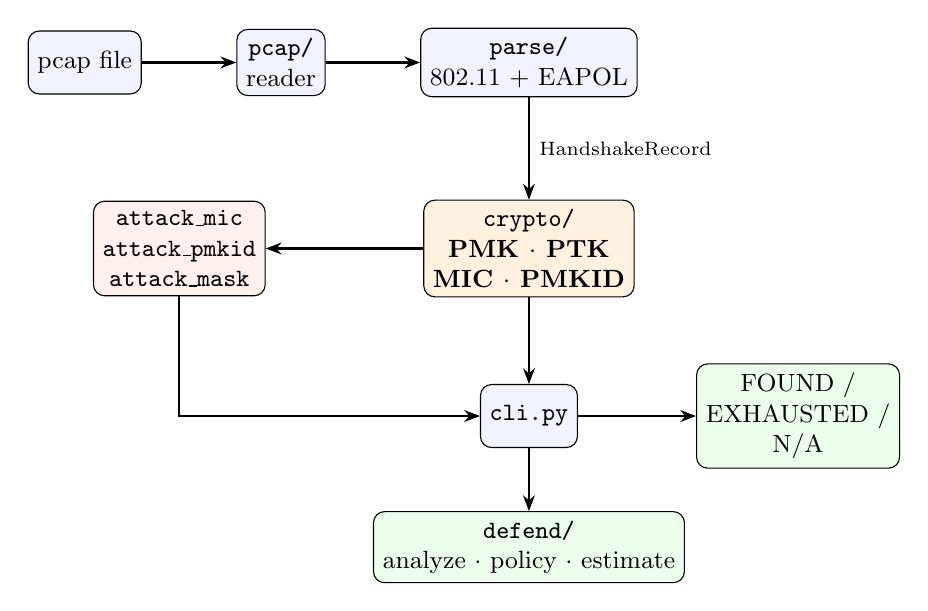
\begin{tikzpicture}[
  node distance=8mm and 12mm,
  box/.style={draw, rounded corners, align=center, minimum height=8mm, font=\small, fill=blue!5},
  core/.style={draw, rounded corners, align=center, minimum height=9mm, font=\small\bfseries, fill=orange!12},
  atk/.style={draw, rounded corners, align=center, minimum height=8mm, font=\small, fill=red!6},
  def/.style={draw, rounded corners, align=center, minimum height=8mm, font=\small, fill=green!8},
  arr/.style={-{Stealth[length=2mm]}, thick}
]
\node[box] (pcap) {pcap file};
\node[box, right=of pcap] (reader) {\code{pcap/}\\reader};
\node[box, right=of reader] (parse) {\code{parse/}\\802.11 + EAPOL};
\node[core, below=13mm of parse] (crypto) {\code{crypto/}\\PMK $\cdot$ PTK\\MIC $\cdot$ PMKID};
\node[atk, left=20mm of crypto] (attacks) {\code{attack\_mic}\\\code{attack\_pmkid}\\\code{attack\_mask}};
\node[box, below=11mm of crypto] (cli) {\code{cli.py}};
\node[def, right=15mm of cli] (verdict) {FOUND /\\EXHAUSTED /\\N/A};
\node[def, below=8mm of cli] (defend) {\code{defend/}\\analyze $\cdot$ policy $\cdot$ estimate};

\draw[arr] (pcap) -- (reader);
\draw[arr] (reader) -- (parse);
\draw[arr] (parse) -- node[right,font=\scriptsize]{HandshakeRecord} (crypto);
\draw[arr] (crypto) -- (attacks);
\draw[arr] (attacks) |- (cli);
\draw[arr] (crypto) -- (cli);
\draw[arr] (cli) -- (verdict);
\draw[arr] (cli) -- (defend);
\end{tikzpicture}
\caption{The pipeline. Only the attack module changes between the three attacks; the file
reader, the 802.11/EAPOL parser, the crypto core, and the CLI are shared. This shared core is
what makes it ``one setup.''}
\label{fig:arch}
\end{figure}

\begin{center}
\small
\begin{tabularx}{\textwidth}{@{}l X@{}}
\toprule
\code{wpacrack/crypto/} & PMK (PBKDF2-HMAC-SHA1), PRF-512/PTK, MIC (KDV~1/2), PMKID --- the shared verifiers \\
\code{wpacrack/pcap/} & \code{pcap} + \code{pcapng} file reader (both byte orders) \\
\code{wpacrack/parse/} & radiotap / 802.11 / EAPOL deframing, RSN IE + AKM, beacon SSID $\to$ \code{HandshakeRecord} \\
\code{wpacrack/attack\_mic/} & Attack~1 driver \\
\code{wpacrack/attack\_pmkid/} & Attack~2 driver \\
\code{wpacrack/attack\_mask/} & Attack~3 driver (mask expansion + time-box) \\
\code{wpacrack/defend/} & \code{analyze.py}, \code{policy.py}, \code{estimate.py} \\
\code{wpacrack/sim/} & synthetic handshake/pcap generator (builds the demo fixtures) \\
\code{wpacrack/cli.py} & unified CLI: \code{mic\,|\,pmkid\,|\,mask\,|\,analyze\,|\,policy\,|\,estimate\,|\,report} \\
\code{tests/} & 16 automated tests (crypto known-answer + integration + real capture) \\
\bottomrule
\end{tabularx}
\end{center}

%======================================================================
\section{Protocol background and where we attack}

WPA2-Personal never sends the passphrase or the derived key over the air. Instead, a station
and access point run a \textbf{4-way handshake} that proves both sides know the Pairwise Master
Key (PMK) and derives fresh session keys. Because the handshake carries values that are a
function of the PMK, an attacker who \emph{captures} the handshake can test passphrase guesses
\emph{offline}: for each guess, derive the PMK and check whether it reproduces a captured value.

\begin{figure}[h]
\centering
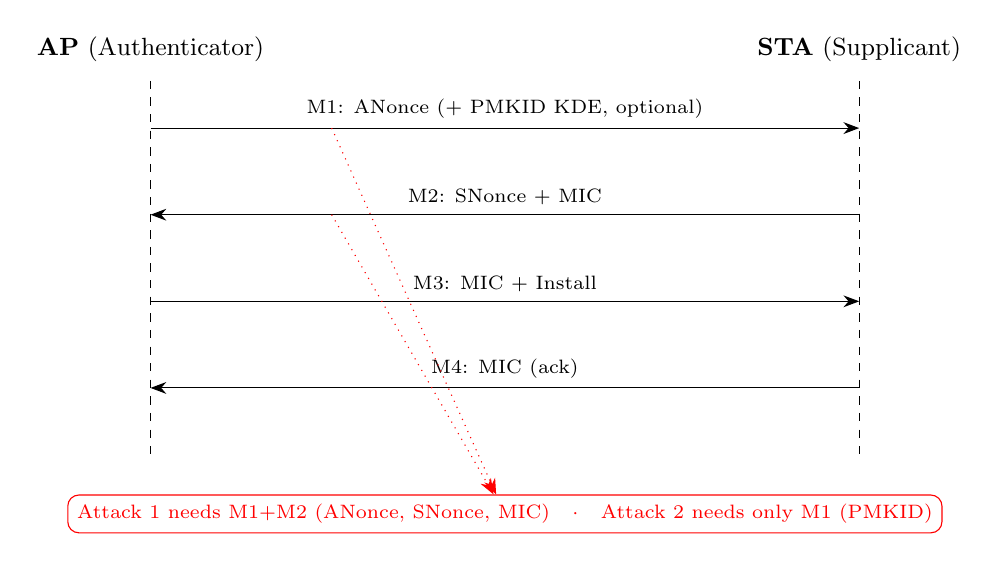
\begin{tikzpicture}[font=\small,>={Stealth[length=2mm]}]
\node (ap) at (0,0) {\textbf{AP} (Authenticator)};
\node (st) at (9,0) {\textbf{STA} (Supplicant)};
\draw[dashed] (0,-0.4) -- (0,-5.2);
\draw[dashed] (9,-0.4) -- (9,-5.2);
\draw[->] (0,-1.0) -- node[above,font=\scriptsize]{M1: ANonce\ (+ PMKID KDE, optional)} (9,-1.0);
\draw[<-] (0,-2.1) -- node[above,font=\scriptsize]{M2: SNonce + MIC} (9,-2.1);
\draw[->] (0,-3.2) -- node[above,font=\scriptsize]{M3: MIC + Install} (9,-3.2);
\draw[<-] (0,-4.3) -- node[above,font=\scriptsize]{M4: MIC (ack)} (9,-4.3);
\node[draw,red,rounded corners,font=\scriptsize,align=center] (tap) at (4.5,-5.9)
  {\textcolor{red}{Attack~1 needs M1{+}M2 (ANonce, SNonce, MIC)\quad$\cdot$\quad Attack~2 needs only M1 (PMKID)}};
\draw[red,->,dotted] (2.3,-1.0) -- (tap);
\draw[red,->,dotted] (2.3,-2.1) -- (tap);
\end{tikzpicture}
\caption{The 4-way handshake as seen in a capture, and which messages each attack needs. We
recover the passphrase from passively captured frames only.}
\label{fig:handshake}
\end{figure}

\noindent The verifiers our \code{crypto/} module implements (one implementation, shared by all
three attacks) are exactly:
\begin{align*}
\text{PMK}   &= \text{PBKDF2-HMAC-SHA1}(\text{passphrase},\ \text{SSID},\ 4096,\ 32)
              \qquad(\text{SSID is the raw salt})\\
\text{PTK}   &= \text{PRF-512}(\text{PMK},\ \text{``Pairwise key expansion''},\
                \min(AA,SPA)\,\|\,\max(AA,SPA)\,\|\,\min(An,Sn)\,\|\,\max(An,Sn))\\
\text{MIC}   &= \text{HMAC}(\underbrace{\text{PTK}[0{:}16]}_{\text{KCK}},\ \text{EAPOL frame with MIC field zeroed})
              \quad(\text{HMAC-MD5 or HMAC-SHA1 by Key Descriptor Version})\\
\text{PMKID} &= \text{HMAC-SHA1}(\text{PMK},\ \text{``PMK Name''}\,\|\,AA\,\|\,SPA)[0{:}16]
\end{align*}
The MIC algorithm is chosen by the Key Descriptor Version field (v1 = HMAC-MD5, v2 =
HMAC-SHA1-128); v3 (AES-128-CMAC, 802.11w) is detected and reported as out of scope for this
standard-library-only tool. All comparisons use \code{hmac.compare\_digest}.

%======================================================================
\section{Demonstration}

All commands below are run from the repository root. There are two kinds of input capture, and
we are careful to distinguish them:
\begin{itemize}
\item \textbf{Synthetic fixtures} (\code{fixtures/*.pcap}) --- built by our own \code{sim/}
      module with \emph{known} passphrases, so every code path (each attack, the negative
      control, the WPA3 case) can be exercised deterministically.
\item \textbf{Real, Internet-sourced captures} (\code{fixtures/public/}) --- published sample
      captures from Wireshark and aircrack-ng, with documented passphrases. These prove the
      tool works on real 802.11 traffic, not just on captures it generated itself.
\end{itemize}
No live or over-the-air capture was performed; that is deliberate and within the approved scope.

\subsection{Built-in self-test on the synthetic fixtures}

\code{python3 -m wpacrack report} regenerates the fixtures, runs all three attacks plus the
negative control and the defense analyzer, and asserts each expected verdict. Real output:

\begin{verbatim}
=== attack results ===
  [PASS] 1 MIC (dict hit)           -> FOUND pw='password123' (tried=3 164/s)
  [PASS] 2 PMKID (dict hit)         -> FOUND pw='password123' (tried=3 180/s)
  [PASS] 3 MASK (6-digit)           -> FOUND pw='001234' (tried=1235 166/s)
  [PASS] 1 MIC (negative control)   -> EXHAUSTED (tried=5 171/s)

=== defense analyzer ===
  [OK-SAE] bssid=02:00:00:00:00:09 WPA3-SAE only: no offline PMK/PMKID target
  [WARN-PSK] bssid=02:00:00:00:00:01 WPA2-PSK: offline dictionary / PMKID attack possible

SELF-TEST: ALL PASS
\end{verbatim}

\subsection{Real, Internet-sourced captures}
\label{sec:realcaps}

This is the strongest evidence that the tool is correct: it recovers the documented passphrase
from four independent, publicly published captures it had no hand in creating. Real output:

\begin{verbatim}
$ wpacrack mic   --pcap fixtures/public/wpa-Induction.pcap --wordlist wl --ssid Coherer
[MIC]   FOUND passphrase='Induction'    (ssid=Coherer,      tried=2, time=0.01s, rate=174/s)

$ wpacrack mic   --pcap fixtures/public/wpa.cap            --wordlist wl
[MIC]   FOUND passphrase='biscotte'     (ssid=test,         tried=2, time=0.01s, rate=174/s)

$ wpacrack mic   --pcap fixtures/public/wpa2.eapol.cap     --wordlist wl --ssid Harkonen
[MIC]   FOUND passphrase='12345678'     (ssid=Harkonen,     tried=2, time=0.01s, rate=172/s)

$ wpacrack pmkid --pcap fixtures/public/test-pmkid.pcap    --wordlist wl
[PMKID] FOUND passphrase='SP-91862D361' (ssid=WLAN-771698,  tried=2, time=0.01s, rate=174/s)
\end{verbatim}

\begin{center}
\begin{tabularx}{\textwidth}{@{}X l l l l@{}}
\toprule
\textbf{Capture (source)} & \textbf{SSID} & \textbf{Attack} & \textbf{Passphrase} & \textbf{Result} \\
\midrule
\code{wpa-Induction.pcap} (Wireshark) & Coherer & 1 (MIC)   & \code{Induction}    & \textcolor{good}{FOUND} \\
\code{wpa.cap} (aircrack-ng)          & test    & 1 (MIC)   & \code{biscotte}     & \textcolor{good}{FOUND} \\
\code{wpa2.eapol.cap} (aircrack-ng)   & Harkonen& 1 (MIC)   & \code{12345678}     & \textcolor{good}{FOUND} \\
\code{test-pmkid.pcap} (aircrack-ng)  & WLAN-771698 & 2 (PMKID) & \code{SP-91862D361} & \textcolor{good}{FOUND} \\
\bottomrule
\end{tabularx}
\end{center}

\noindent The \code{test-pmkid.pcap} case is notable: it has \emph{no} 4-way handshake at all,
only a Message~1 carrying a PMKID. Attack~2 cracks it anyway, while Attack~1 correctly reports
that it cannot run --- exactly the honest behaviour we want:

\begin{verbatim}
$ wpacrack mic --pcap fixtures/public/test-pmkid.pcap --wordlist wl
[MIC] N/A  (ssid=WLAN-771698, no usable M1+M2 / M2+M3 handshake)
\end{verbatim}

\subsection{Attack 3 in detail: mask patterns beyond digits}

The self-test above uses the mask \code{?d?d?d?d?d?d} (six digits) purely so it finishes in
under a second. That is one instance of a general mask engine: a mask is a string of tokens
--- \code{?d} digit, \code{?l} lower, \code{?u} upper, \code{?s} symbol, \code{?a} = all of
those, plus literal characters and \code{??} for a literal question mark --- and each position
expands to its character set. To show it is not digits-only, here is a real run against a
synthetic capture whose passphrase is \code{wifiAb37} (8 characters), cracked with a mask that
mixes literals with upper, lower, and digit tokens:

\begin{verbatim}
$ wpacrack mask --pcap fixtures/hs_mask_mixed.pcap --mask 'wifi?u?l?d?d' --ssid demoAP --timebox 120
[MASK] FOUND passphrase='wifiAb37' (ssid=demoAP, tried=138, time=0.92s, rate=150/s,
       mask=wifi?u?l?d?d, keyspace=67,600)
\end{verbatim}

\noindent A mask attack can only be \emph{demonstrated} on a small keyspace: the demo masks
above have keyspaces of $10^{6}$ and $6.8\times10^{4}$, found in seconds. A full unknown 8-char
mixed mask (\code{?a} $\times 8$) is $6.6\times10^{15}$ candidates --- infeasible in demo time,
and indeed infeasible in general, which is exactly the point the defense section
(\S\ref{sec:defense}) quantifies. The value of the mask attack is that it targets \emph{known
structure} (a numeric PIN, a fixed prefix, a known length) far more cheaply than a generic
wordlist.

\subsection{Was it successful, and why (or why not)?}

Yes, in every case where the passphrase is reachable, and it correctly fails (without a false
positive) where it is not:
\begin{itemize}
\item \textbf{Attack~1 (MIC)} succeeds whenever the capture contains a usable handshake pairing
      (M1+M2 or M2+M3) \emph{and} the passphrase is in the wordlist --- confirmed on three real
      captures above.
\item \textbf{Attack~2 (PMKID)} succeeds whenever Message~1 carries a PMKID and the passphrase
      is in the wordlist --- confirmed on a real capture with no full handshake.
\item \textbf{Attack~3 (mask)} succeeds when the passphrase matches the mask pattern within the
      time-box --- confirmed both on a 6-digit numeric mask (\code{001234}) and on a mixed
      upper/lower/digit mask (\code{wifiAb37}), using the same mask engine.
\item \textbf{It fails safely} when it should: a wrong wordlist yields \code{EXHAUSTED} (never a
      bogus \code{FOUND}), and a missing field yields \code{N/A}.
\end{itemize}
The reason it works is purely that WPA2-PSK exposes a PMK-derived value (the MIC or the PMKID)
to anyone who captures the handshake, so guessing is an offline computation. The reason it
\emph{cannot} succeed against a strong passphrase is the size of the keyspace, quantified in
Section~\ref{sec:defense}.

%======================================================================
\section{Observed output on attacker, victim, and other hosts}

Because this is an offline attack on a captured file, the ``hosts'' picture is different from a
live attack, and we state it plainly rather than staging a fake victim screen:
\begin{itemize}
\item \textbf{Attacker host:} the console output shown throughout Section~4 --- the parsed
      handshake fields (SSID, BSSID, station MAC), the number of candidates tried, the elapsed
      time and rate, and finally the recovered passphrase or a clean \code{EXHAUSTED}/\code{N/A}.
\item \textbf{Victim / AP / other hosts:} \emph{none, during the attack.} The attack is entirely
      offline; nothing is transmitted, so no live victim or third-party host observes anything.
      The only ``victim-side'' artifact is the captured \code{pcap} itself, which was produced
      before and independently of our tool (a published sample capture, or our own synthetic
      generator). This is the honest consequence of the supervisor-approved, pcap-only scope.
\end{itemize}

%======================================================================
\section{Performance: estimated rate vs.\ measured experiment}
\label{sec:perf}

The design proposal estimated crack times from a single \emph{assumed} candidate rate that was
never measured. We closed that gap by actually measuring the rate --- on CPU, and on GPU with
our own PBKDF2-HMAC-SHA1 kernel written in PyTorch (RFC~2898 / IEEE~802.11i --- again, not
aircrack-ng or Hashcat). That kernel is a separate experimental artifact under \code{notebooks/}
and is validated byte-for-byte against \code{hashlib.pbkdf2\_hmac} before any timing is trusted;
it does not change the stdlib-only tool. Measurements below are from a Kaggle instance with two
Tesla~T4 GPUs.

\begin{figure}[h]
\centering
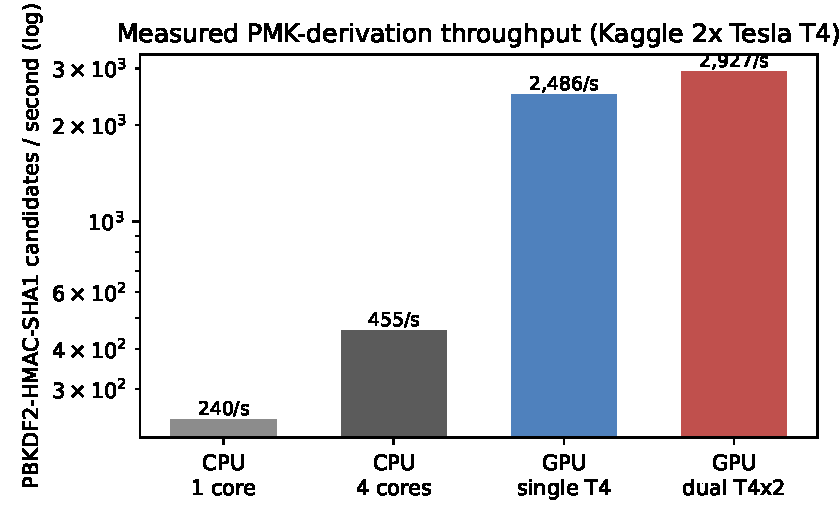
\includegraphics[width=0.60\textwidth]{figures/throughput.pdf}
\caption{Measured PBKDF2-HMAC-SHA1 throughput: from 240 candidates/s on a single CPU core up to
2{,}927 candidates/s across two T4 GPUs --- a $12.2\times$ speedup on the same host. PBKDF2's
4096 iterations per candidate are essentially the entire cost of every attack.}
\label{fig:throughput}
\end{figure}

\subsection{The GPU does not always win: a measured crossover}

Our GPU kernel has a fixed per-call overhead, so at small candidate counts a plain CPU is
actually faster; the GPU only wins above a break-even size. We measured this directly on a real
capture (\code{wpa2.eapol.cap}) rather than assuming it:

\begin{figure}[h]
\centering
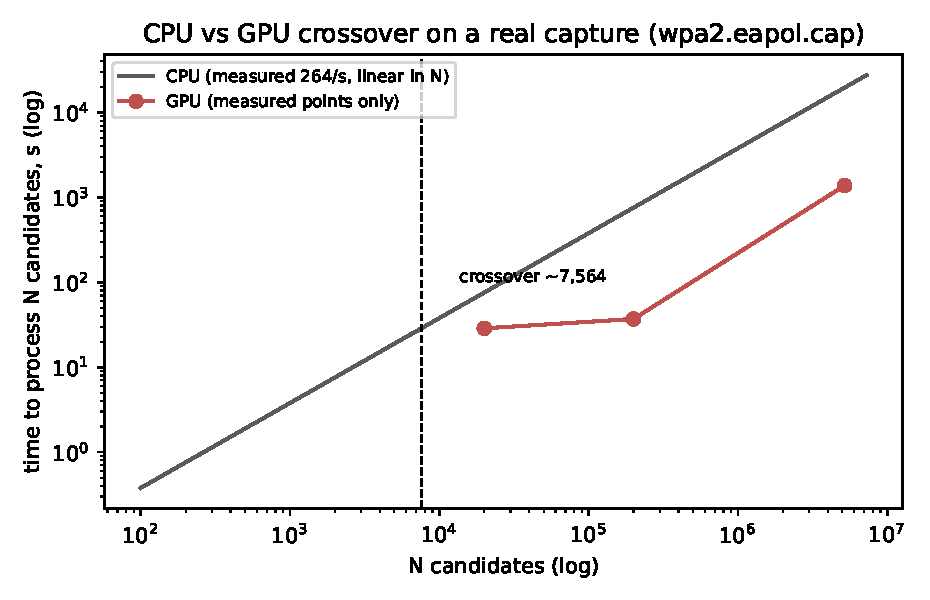
\includegraphics[width=0.62\textwidth]{figures/crossover.pdf}
\caption{CPU time grows linearly with the wordlist size $N$ (constant cost per candidate); the
GPU's three measured points do not. They cross at roughly 7{,}564 candidates: below that, plain
CPU wins; above it, the GPU wins by an increasingly large margin.}
\label{fig:crossover}
\end{figure}

\subsection{Full-scale result on a realistic wordlist}

The headline measurement is a genuine, realistic-scale run: SecLists' full 5{,}189{,}454-entry
common-password list against \code{wpa2.eapol.cap}, scanned to complete exhaustion (the real
passphrase was excluded first so neither side could stop early).

\begin{center}
\begin{tabularx}{\textwidth}{@{}l r r X@{}}
\toprule
\textbf{Run} & \textbf{Candidates} & \textbf{Time} & \textbf{Basis} \\
\midrule
GPU, dual T4x2 & 5{,}189{,}454 & 23.0 min & \textbf{measured} (executed on Kaggle) \\
CPU, 1 core    & 5{,}189{,}454 & 5.5 h    & calculated ($N/\text{measured }264\text{/s}$), not re-run \\
CPU, this machine (MIC)   & 99{,}999  & 11.5 min & measured, independent 2nd machine (144/s) \\
CPU, this machine (PMKID) & 100{,}000 & 9.5 min  & measured, independent 2nd machine (175/s) \\
\bottomrule
\end{tabularx}
\end{center}

\noindent The dual-GPU run of the full realistic list completed a real crack attempt in
\textbf{23 minutes}; the single-core CPU equivalent is \emph{calculated} at $\sim$5.5 hours (we
do not re-run it, because PBKDF2's cost per candidate is constant, so $N/\text{rate}$ is exact).
The two ``this machine'' rows are a real, independently executed cross-check on a second
computer, against two different real captures and both attack types --- confirming the CPU rate
is not a one-machine artifact. Below the $\sim$7{,}564-candidate crossover, however, plain CPU is
the right tool: for the small dictionaries and short masks in our own demo (Section~4), CPU is
not merely adequate, it is faster than the unoptimized GPU kernel.

%======================================================================
\section{Defense (countermeasure)}
\label{sec:defense}

We built the countermeasure into the same tool, as three defensive subcommands.

\textbf{1. Network analyzer (\code{analyze}).} Reads the RSN AKM suite from a beacon and gives a
verdict: WPA2-PSK $\Rightarrow$ \textcolor{warn}{offline-crackable}; WPA3 transition mode
$\Rightarrow$ \textcolor{warn}{WPA2 fallback still crackable}; WPA3-SAE-only $\Rightarrow$
\textcolor{good}{no offline target}. On the real \code{wpa2.eapol.cap} beacon:
\begin{verbatim}
$ wpacrack analyze --pcap fixtures/public/wpa2.eapol.cap
[ANALYZE] WARN-PSK  bssid=00:14:6c:7e:40:80 akms=[2]  WPA2-PSK: offline dictionary / PMKID attack possible
\end{verbatim}

\textbf{2. Passphrase policy (\code{policy}).} Flags short, low-diversity, or common-list
passphrases. Real output for a weak and a strong passphrase:
\begin{verbatim}
$ wpacrack policy --passphrase "password123"
passphrase policy: WEAK (length 11)
  - shorter than 15 characters (recommend >= 15 for WPA2-PSK)
  - uses fewer than 3 character classes
  - appears in a common-password list

$ wpacrack policy --passphrase "correct horse battery staple 9!"
passphrase policy: STRONG (length 31)
  - meets length and character-class guidance; keep it unique and unguessable
\end{verbatim}

\textbf{3. Crack-time estimator (\code{estimate}).} Uses our \emph{measured} fastest rate
(2{,}927 cand/s, dual T4) to show what actually survives an offline attack. This is real
\code{estimate} output; the ``expected'' column is half the keyspace divided by the rate:

\begin{center}
\begin{tabularx}{\textwidth}{@{}X r r l@{}}
\toprule
\textbf{Passphrase shape} & \textbf{Keyspace} & \textbf{Expected crack time} & \textbf{Verdict} \\
\midrule
6 digits            & $10^{6}$              & 2.8 minutes   & \textcolor{warn}{WEAK} \\
8 digits            & $10^{8}$              & 4.7 hours     & \textcolor{warn}{WEAK} \\
8 lowercase letters & $2.1\times10^{11}$    & 1.1 years     & OK \\
8 full-ASCII chars  & $6.6\times10^{15}$    & $\sim$35{,}900 years & \textcolor{good}{OK} \\
12 full-ASCII chars & $5.4\times10^{23}$    & $\sim 3\times10^{12}$ years & \textcolor{good}{OK} \\
15 full-ASCII chars & $4.6\times10^{29}$    & $\sim 2.5\times10^{18}$ years & \textcolor{good}{OK} \\
\bottomrule
\end{tabularx}
\end{center}

\begin{figure}[h]
\centering
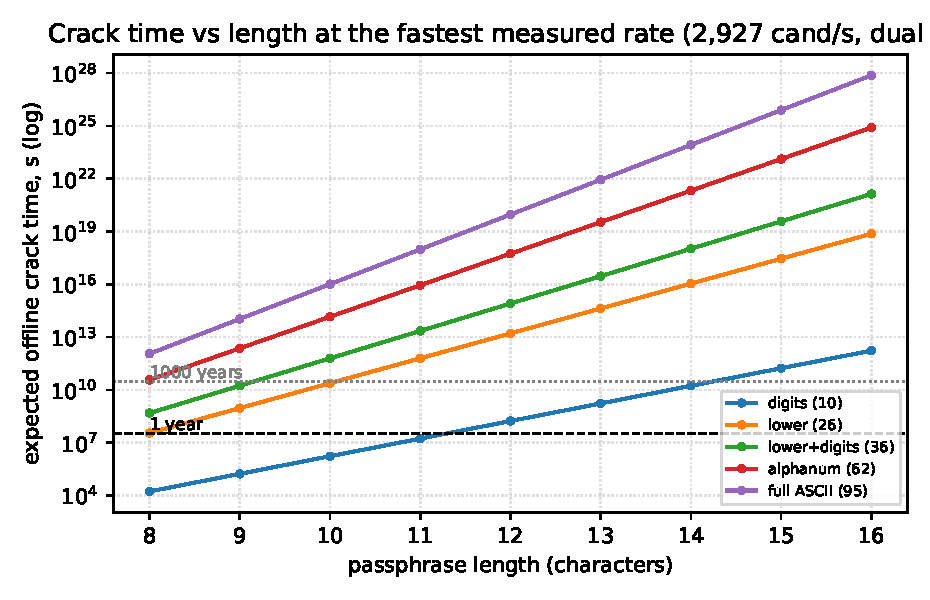
\includegraphics[width=0.62\textwidth]{figures/timecrack.pdf}
\caption{Expected offline crack time vs.\ passphrase length, per character set, at the fastest
rate we measured (2{,}927 cand/s). Short or single-class passphrases fall below the one-year
line; a long mixed passphrase is astronomically infeasible even with a GPU.}
\label{fig:timecrack}
\end{figure}

\noindent\textbf{Recommendation.} Use a long ($\geq 15$ character) mixed passphrase that is not
in any wordlist; prefer WPA3-SAE-only and disable WPA2 transition mode (SAE / Dragonfly exposes
no PMK-derived value to an offline capture); and keep SAE implementations patched against the
Dragonblood class of attacks (Vanhoef \& Ronen, 2020). Crucially, the length recommendation
holds \emph{regardless} of whether the attacker uses a CPU or a GPU --- the keyspace of a long
passphrase dwarfs any realistic hardware speedup.

%======================================================================
\section{Correctness and honesty of the demonstration}

\begin{itemize}
\item \textbf{Known-answer vector.} Our PMK matches the canonical IEEE~802.11i value for
      (\code{password}, \code{IEEE}):
      \code{f42c6fc52df0ebef9ebb4b90b38a5f902e83fe1b135a70e23aed762e9710a12e}.
\item \textbf{Real captures.} The full PMK$\to$PTK$\to$MIC and PMK$\to$PMKID paths recover the
      documented passphrases from four independent public captures (Section~\ref{sec:realcaps}),
      proving the code matches real 802.11 and not merely our own generator.
\item \textbf{Automated tests.} \code{pytest} runs \textbf{16 tests, all passing} (6 crypto
      known-answer tests, 9 integration tests, 1 real-capture test).
\item \textbf{No false positives.} The negative-control scenario searches a wrong wordlist over
      a valid handshake and returns \code{EXHAUSTED}, never a bogus \code{FOUND}; all comparisons
      are constant-time full-digest checks.
\item \textbf{Scope guard.} \code{tools/ethics\_guard.py} fails the build if any socket,
      injection, or raw-transmit code appears anywhere in \code{wpacrack/}; it currently passes
      (\emph{``ETHICS GUARD PASSED: wpacrack/ is file-in / verdict-out only.''}).
\end{itemize}

%======================================================================
\section{Reproducibility}
\label{sec:repro}

Every result in this report is reproducible from the repository root:
\begin{verbatim}
python3 -m wpacrack.sim                              # (re)build the synthetic fixtures
python3 -m wpacrack report --fixtures fixtures       # the Section-4.1 self-test
bash tools/fetch_samples.sh                          # download the public captures
python3 -m wpacrack mic   --pcap fixtures/public/wpa-Induction.pcap --wordlist WL --ssid Coherer
python3 -m wpacrack pmkid --pcap fixtures/public/test-pmkid.pcap    --wordlist WL
python3 -m wpacrack analyze  --pcap fixtures/public/wpa2.eapol.cap
python3 -m wpacrack policy   --passphrase "password123"
python3 -m wpacrack estimate --charset a --length 12 --rate 2927
# mixed-charset mask demo (Section 4.3): build a small fixture, then crack with ?u ?l ?d tokens
python3 -c "from wpacrack import sim; sim.build_capture('fixtures/hs_mask_mixed.pcap','demoAP','wifiAb37',messages=(1,2))"
python3 -m wpacrack mask --pcap fixtures/hs_mask_mixed.pcap --mask 'wifi?u?l?d?d' --ssid demoAP --timebox 120
python -m pytest -q                                  # 16 tests (in a venv)
python3 tools/ethics_guard.py                        # scope guard
python3 report/make_figures.py                       # regenerate this report's figures
\end{verbatim}
The GPU measurements (Section~\ref{sec:perf}) are reproduced by the two notebooks under
\code{notebooks/} on a Kaggle GPU instance; each begins with a validation cell that must pass
before any timing is trusted.

\vspace{1em}
\noindent\small\textit{Contributions: both group members (2105088, 2105066) contributed to the
design, implementation, and testing; see the repository commit history for detailed authorship.
References: IEEE~Std~802.11i-2004; RFC~2898 / RFC~8018 (PBKDF2); He \& Mitchell, NDSS~2005
(4-way handshake analysis); CERT-EU~SA2018-019 (PMKID attack); RFC~7664 and Lancrenon \&
\v{S}krobot, ISC~2015 (Dragonfly/SAE); Vanhoef \& Ronen, IEEE~S\&P~2020 (Dragonblood).}

\end{document}
